%-----------------------------------------------------------------------
% Installation : M2eclipse
% 
%-----------------------------------------------------------------------
%\newpage

%-----------------------------------------------------------------------
\section{Installation du plugin M2eclipse dans Eclipse}

GeOxygene est généré à partir de Maven\footnote{http://maven.apache.org/}.  Le projet m2eclipse fournit un support afin d'utiliser les fonctionnalités de Maven dans l'éditeur Eclipse.

\medskip

\noindent
L'intégration Maven pour Eclipse est séparée en deux plugins : le core et un module optionnel contenant des composants supplémentaires. Pour installer GeOxygene, il faut les deux.


\subsection{m2eclipse Core Components}
Reprenez les 8 premières étapes de l'installation du plugin subeclipse mais en adaptant les paramètres.

\medskip

\noindent
1. A l'étape 3 saisir :\\

\begin{tabular}[!t]{ll}
{\bf Name : }&{m2eclipse}\\
{\bf Location : }&{\href{http://m2eclipse.sonatype.org/sites/m2e}{http://m2eclipse.sonatype.org/sites/m2e}}\\
\end{tabular}\\

\smallskip
\begin{center}
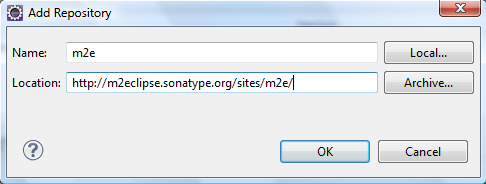
\includegraphics[width=0.4\linewidth]{../../resources/images/guide_installation/m2eclipseUrl.png}
\end{center}

\noindent
2. A l'étape 4 choisir l'unique composant "Maven Integration for Eclipse".\\
\begin{center}
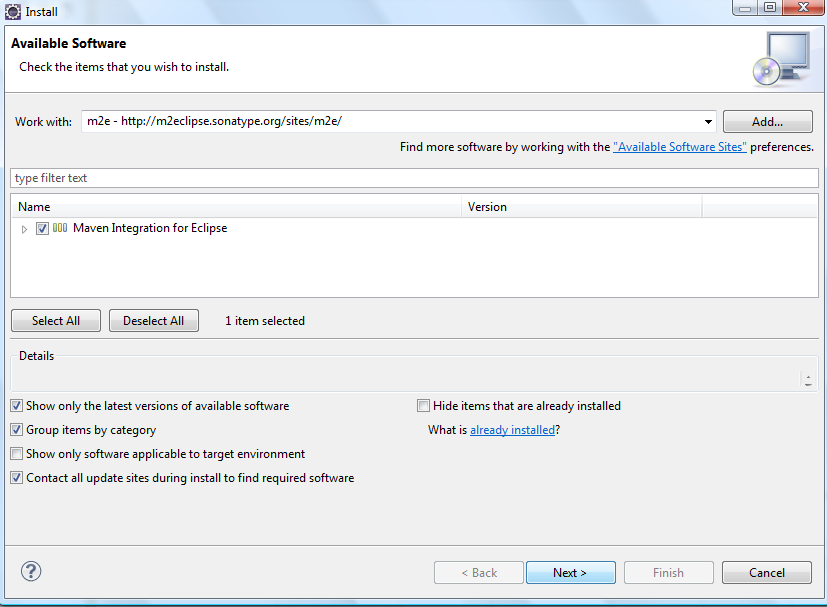
\includegraphics[width=0.4\linewidth]{../../resources/images/guide_installation/m2eclipseEtape1.png}
\end{center}

\noindent
3. A l'étape 8, une fois l'installation terminée, une fenêtre propose de redémarrer Eclipse, inutile de le faire à ce stade.




%-----------------------------------------------------------------------
%\newpage

\subsection{m2eclipse Extras}
Une dès options disponibles dans ce plugin est la possibilité d'importer directement d'un dépôt SVN un projet Maven. C'est celui que l'on va installer.

\medskip

\noindent
Reprenez une nouvelle fois les 8 premières étapes de l'installation du plugin subeclipse mais en adaptant les paramètres.

\newpage

\noindent
1. A l'étape 3 saisir :\\

\begin{tabular}[!t]{ll}
{\bf Name : }&{m2e-extras}\\
{\bf Location : }&{\href{http://m2eclipse.sonatype.org/sites/m2e-extras}{http://m2eclipse.sonatype.org/sites/m2e-extras}}\\
\end{tabular}\\

\smallskip
\begin{center}
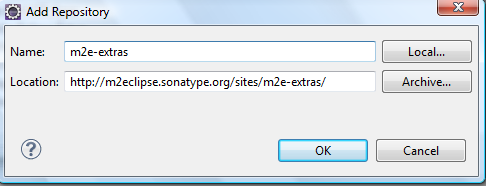
\includegraphics[width=0.4\linewidth]{../../resources/images/guide_installation/m2eclipseExtrasUrl.png}
\end{center}

\noindent
2. A l'étape 4 sélectionner au moins le composant "Maven SCM handler for Subclipse".\\
\begin{center}
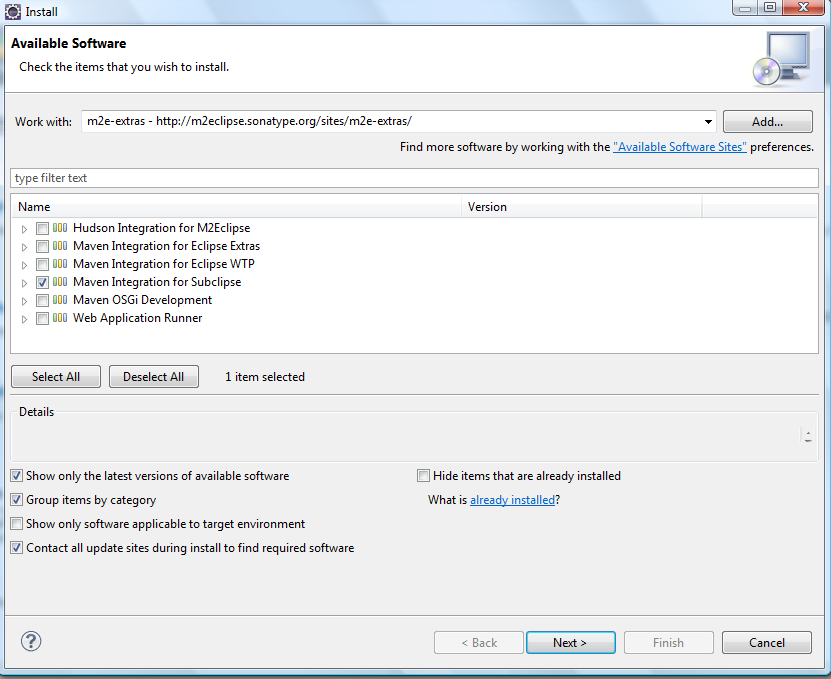
\includegraphics[width=0.4\linewidth]{../../resources/images/guide_installation/m2eclipseExtrasEtape1.png}
\end{center}

\noindent
3. A l'étape 8, une fois l'installation terminée, une fenêtre propose de redémarrer Eclipse, à ce stade il est vivement conseillé de le faire.





